%%%%%%%%%%%%%%%%%%%%%%%%%%%%%%%%%%%%%%%%%%%%%
%%%%%%%%%%%%%%%%%%%%%%%%%%%%%%%%%%%%%%%%%%%%%
%%%%%%%%%%%%%%%%%%%%%%%%%%%%%%%%%%%%%%%%%%%%%
%%%%%%%%%%%%%%%%%%%%%%%%%%%%%%%%%%%%%%%%%%%%%
\section{The Reeb coordinates of a braid variety}\label{sec:Reeb_variables} Let $\beta\in\brn$ be a positive braid word with length $\ell:=\ell(\beta)$. By \Cref{def:braid_variety}, the braid variety $X(\beta)$ is defined as a subvariety of the projective variety $(\G/\borel)^{\ell(\beta)+1}$. The description of $X(\beta)$ in \cref{def:braid_variety} and discussions above are coordinate-free. There is nevertheless some merit in introducing explicit coordinates to study $X(\beta)$. In this section we introduce a particular set of coordinates in $\mathbb{A}_\kk^{\ell(\beta)}$ and describe a particular embedding $X(\beta)\sse\mathbb{A}_\kk^{\ell(\beta)}$ as an affine subvariety using such coordinates. We refer to such coordinates as Reeb coordinates or $z$-variables, as they are geometrically motivated by the study of Reeb chords in contact topology, see \cite[Section 5.1]{CasalsNg22}.\\

Because of their geometric origin and several facts stemming from contact and symplectic topology, these Reeb coordinates have remarkable properties to study braid varieties. A few advantages that Reeb coordinates have are:

\begin{enumerate}

    \item All the cluster variables $\{A^\w_v\}$ associated to any weave $\w:\beta\lr\delta(\beta)$ will be polynomials in the Reeb $z$-coordinates $(z_1,\ldots,z_\ell)$, $\ell=\ell(\beta)$, cf.~\Cref{thm:polynomiality}. In addition, the exponents in the leading monomial of such a polynomial $A^\w_v(z_1,\ldots,z_\ell)$, in the lexicographic order given by $z_1\prec z_2\prec \ldots\prec z_\ell$, provide the crystal vertex in the $\beta$-Lusztig parametrization of a global basis of $\kk[X(\beta)]$, see e.g.~\Cref{thm:leading_monomial_cluster_A_variables}. Plus, there is a combinatorial expression for such polynomials $A^\w_v(z_1,\ldots,z_\ell)$ in terms of a hook content formula, cf.~\Cref{thm:hook_content_cluster_A_variables}.\\
    
    \item The proof that the inclusion \cref{eq:inclusion_cluster_algebra} is an equality provided in \cite[Section 5]{CGGLSS25} uses Reeb coordinates. In addition, proofs obtained by computations in Reeb coordinates work identically for all $\G$. For instance, some invariance properties directly transfer from $\SL_3$ to $\G$ via pinnings, and having explicit coordinate-dependent equations for $X(\beta)$ as an algebraic subvariety of $\mathbb{A}_\kk^{\ell(\beta)}$ can help study properties of $X(\beta)$ such as smoothness, dimension, group actions, and Gr\"obner bases for $\kk[X(\beta)]$, among others. In particular, the torus action on braid varieties has a neat expression in terms of Reeb coordinates, cf.~\Cref{lem:torusaction_coordinates}, as does the cluster 2-form, cf.~\Cref{prop:2forms}. Similarly, the superpotential of a natural log Calabi-Yau compactification of $X(\beta)$ has a remarkably simple expression in the Reeb coordinates, cf.~\Cref{thm:superpotential_Reeb_coordinates}.\\
    
    \item For everyday use, it is also often useful in applications to have explicit formulas for the cluster variables $\{A^\w_v\}$ in terms of a specific set of generators for $\kk[X(\beta)]$. In particular, there is computer software available to compute cluster variables from Demazure weaves which uses this explicit Reeb coordinate system.\footnote{A Javascript applet is available at \href{https://daping-weng.github.io/math/demazure_weave.html}{Daping Weng's website here}.}
\end{enumerate}

%%%%%%%%%%%%%%%%%%%%%%%%%%%%%%%%%%%%%%%%%%%%%
%%%%%%%%%%%%%%%%%%%%%%%%%%%%%%%%%%%%%%%%%%%%%
%%%%%%%%%%%%%%%%%%%%%%%%%%%%%%%%%%%%%%%%%%%%%
\subsection{Reeb coordinates for braid varieties}\label{ssec:Reeb_coordinates_braid_variety} We will now consider ambient affine coordinates in $\mathbb{A}_\kk^{\ell}=\Spec k[z_1,\ldots,z_\ell]$ and an embedding $X(\beta)\sse \mathbb{A}_\kk^{\ell}$ with explicit equations cutting out $X(\beta)$ in terms of these $z$-variables. These ambient $z$-variables will also be referred to as Reeb coordinates, and they are closely related to the $\widetilde{z}$-variables in \Cref{lem:framing_variables}. As before, we fix a pinning of the group $\G$ as in \Cref{ssec:rational_functions} and consider
\[
s_{i} := \varphi_{i}\left(\begin{matrix}0 & -1 \\ 1 & 0 \end{matrix} \right)\in \G,
\]
so $s_{i} \in N_{\G}(T)$ lifts the simple reflection corresponding to $i \in \dynkin$. Given a permutation $v\in W(\G)$, we define its lift to $\G$ by choosing an arbitrary reduced expression and multiplying these elements $s_i$ accordingly. In order to discuss tuples of flags, we introduce a variable $z \in k$ and define
\[
B_{i}(z):= x_{i}(z)s_{i} = \varphi_{i}\left(\begin{matrix} z & -1 \\ 1 & 0\end{matrix}\right) \in \G.
\]

\noindent {\it What is this variable $z$ parametrizing in terms of flags?} Suppose we fix a flag $x\borel \in \G/\borel$ and we want to parametrize all flags in $\G/\borel$ which are in relative $s_i$-position with $x\borel$. The claim is that this set is isomorphic to $\mathbb{A}_k^1$ and $z$ provides a coordinate for it. Explicitly, we can parametrize this set via
\begin{equation}\label{eq:Biz_parametrizing_flags_rel_pos}
\{y\borel \in \G/\borel \mid x\borel \buildrel s_{i} \over \longrightarrow y\borel\}\cong \{xB_{i}(z)\borel | z \in \kk\},
\end{equation}
and so two flags $xB_i(z)\borel=xB_i(z')\borel$ are equal if and only if $z=z'$. This is essentially \Cref{lem:framing_variables} for unframed flags.

\begin{example} (1). For $\G=\SL_n$, we choose the following pinning and $B_i(z)$ matrices:
\begin{equation}\label{eq:pinning1}
x_{i}(z) = \begin{pmatrix}
1 & \cdots  & & & \cdots & 0\\
\vdots & \ddots & & & & \vdots\\
0 & \cdots & 1 & z & \cdots & 0\\
0 & \cdots & 0 & 1 & \cdots & 0\\
\vdots &  & & &\ddots & \vdots\\
0 & \cdots & & & \cdots & 1\\
\end{pmatrix},\qquad
y_{i}(z) = \begin{pmatrix}
1 & \cdots  & & & \cdots & 0\\
\vdots & \ddots & & & & \vdots\\
0 & \cdots & 1 & 0 & \cdots & 0\\
0 & \cdots & z & 1 & \cdots & 0\\
\vdots &  & & &\ddots & \vdots\\
0 & \cdots & & & \cdots & 1\\
\end{pmatrix},
\end{equation}
\begin{equation}\label{eq:pinning1}
\chi_{i}(t) = \begin{pmatrix}
1 & \cdots  & & & \cdots & 0\\
\vdots & \ddots & & & & \vdots\\
0 & \cdots & t & 0 & \cdots & 0\\
0 & \cdots & 0 & t^{-1} & \cdots & 0\\
\vdots &  & & &\ddots & \vdots\\
0 & \cdots & & & \cdots & 1\\
\end{pmatrix},\qquad
B_{i}(z) = \begin{pmatrix}
1 & \cdots  & & & \cdots & 0\\
\vdots & \ddots & & & & \vdots\\
0 & \cdots & z & -1 & \cdots & 0\\
0 & \cdots & 1 & 0 & \cdots & 0\\
\vdots &  & & &\ddots & \vdots\\
0 & \cdots & & & \cdots & 1\\
\end{pmatrix},
\end{equation}
where the $(2\times 2)$-submatrices sit at the $i$th and $(i + 1)$st rows and columns. The variable $z$ is thus the $(i,i+1)$-entry of $x_i(z)$, the $(i+1,i)$-entry of $y_i(z)$, and the $(i,i)$-entry of $B_i(z)$. The variable $t$ is the $(i,i)$-entry of $\chi_i(t)$. Note that $B_i(z)^{-1}=s_iB_i(-z)s_i$.\\

\noindent (2) Consider $\G=\SL_2$, and the standard flag $\borel$, which is determined by the line $\borel^1=\langle e_1\rangle\in k^2$. Then the Borel subgroup
$$B_1(z)\borel=\left\{g\in\SL_2: g=\begin{pmatrix}
z & -1\\
1 & 0
\end{pmatrix}B\begin{pmatrix}
0 & 1\\
-1 & z
\end{pmatrix},\mbox{ for some }B\mbox{ upper-triangular}\right\}$$
corresponds (i.e.~it is the stabilizer of) the unique full flag in $k^2$ whose 1-dimensional subspace is $\langle ze_1+e_2\rangle$. Thus $(B_1(z)\borel)^1=\langle ze_1+e_2\rangle$. In particular, since $e_1$ is never parallel to $ze_1+e_2$ for $z\in k$, these two flags are different, i.e.~$\borel\stackrel{s_1}{\to}B_1(z)\borel$. Conversely, any line in $k^2$ which is different from $\langle e_1\rangle$ has a unique generator of the form $ze_1+e_2\in k^2$, and thus $z\in k$ bijectively parametrizes such flags.\sbs
\end{example}

%%%%%%%%%%%%%%%%%%%%%%%%%%%%%%%%%%%%%%%%%%%%%
%%%%%%%%%%%%%%%%%%%%%%%%%%%%%%%%%%%%%%%%%%%%%
%%%%%%%%%%%%%%%%%%%%%%%%%%%%%%%%%%%%%%%%%%%%%
\subsection{Equations for braid varieties via the Reeb coordinates}\label{ssec:equation_braid_varieties_Reeb_coordinates} Given a positive braid word $\beta = \sigma_{i_{1}}\cdots \sigma_{i_{\ell}}$, we define $B_{\beta}(z)\in\G$ as
\begin{equation}\label{eq:braid_matrix}
B_{\beta}(z) := B_{i_{1}}(z_1)\cdots B_{i_{\ell}}(z_\ell) \in \G,\quad z=(z_1,\ldots,z_\ell)\in \mathbb{A}_\kk^{\ell}.
\end{equation}

\noindent As above, these variables $(z_1,\ldots,z_\ell)\in \mathbb{A}_\kk^{\ell}$ associated to the crossings of $\beta$ will be referred to as the $z$-variables or Reeb coordinates for $\beta$. It follows from \cref{eq:Biz_parametrizing_flags_rel_pos} that, in these $z$-coordinates, the braid variety $X(\beta)$ can be described as follows:

\begin{lemma}[\color{blue}Equations for braid varieties in Reeb coordinates\color{black}]\label{lem:equations_braidvar}
Let $\beta = \sigma_{i_{1}}\cdots \sigma_{i_{\ell}}$ be a positive braid word, with Demazure product $\delta(\b)$, and $\delta(\b)^{-1}$ a lift of the inverse of $\delta(\b)$ to $\G$ using $s_i$. Then there is an isomorphism
\begin{equation}\label{eq:braid_var_eq}
X(\beta) \cong \{(z_1, \dots, z_\ell) \in \mathbb{A}_\kk^{\ell} \mid \delta(\b)^{-1}B_{i_{1}}(z_1)\cdots B_{i_{\ell}}(z_\ell) \in \borel\},
\end{equation}
$X(\beta)$ is a smooth irreducible affine variety, and $\dim_\kk(X(\beta))=\ell(\b)-\ell(\delta(\b))$.
\sbs
\end{lemma}

\noindent See \cite[Corollary 3.7]{CGGLSS25} for a detailed proof. The equation $\delta^{-1}B_{i_{1}}(z_1)\cdots B_{i_{r}}(z_r) \in \borel$ is given by the vanishing of some generalized minors, and thus $X(\beta)$ is indeed an affine variety defined over $\Z$. In these $z$-coordinates, the braid invariance properties from \cref{lem:braid_invariance} follow from the identities
$$B_{i}(z)B_{j}(w) = B_{j}(w)B_{i}(z),\quad i,j\in\dynkin\mbox{ not adjacent}$$
$$B_{i}(z_1)B_{j}(z_2)B_{i}(z_3) = B_j(z_3)B_i(z_1z_3 - z_2)B_j(z_1),\quad i,j\in\dynkin\mbox{ adjacent}.$$
The latter is proven by directly transporting the $\SL_3$-identity
$$B_{1}(z_1)B_{2}(z_2)B_{1}(z_3) = B_2(z_3)B_1(z_1z_3 - z_2)B_2(z_1)$$
to $\G$ via pinnings. This $\SL_3$-identity is checked by hand:
$$\begin{pmatrix}
z_1 & -1 & 0\\
1 & 0 & 0\\
0 & 0 & 1\\
\end{pmatrix}
\begin{pmatrix}
1 & 0 & 0\\
0 & z_2 & -1\\
0 & 1 & 0\\
\end{pmatrix}
\begin{pmatrix}
z_3 & -1 & 0\\
1 & 0 & 0\\
0 & 0 & 1\\
\end{pmatrix}=\begin{pmatrix}
z_1z_3-z_2 & -z_1 & 1\\
z_3 & -1 & 0\\
1 & 0 & 0\\
\end{pmatrix},$$
$$\begin{pmatrix}
1 & 0 & 0\\
0 & z_3 & -1\\
0 & 1 & 0\\
\end{pmatrix}
\begin{pmatrix}
z_1z_3-z_2 & -1 & 0\\
1 & 0 & 0\\
0 & 0 & 1\\
\end{pmatrix}
\begin{pmatrix}
1 & 0 & 0\\
0 & z_1 & -1\\
0 & 1 & 0\\
\end{pmatrix}=\begin{pmatrix}
z_1z_3-z_2 & -z_1 & 1\\
z_3 & -1 & 0\\
1 & 0 & 0\\
\end{pmatrix}.
$$
\normalsize
\noindent The cyclic symmetry mentioned in \Cref{sssec:braid_variety_further_symmetries} can also be verified through matrix computation, cf.~\cite[Lemma 3.10]{CGGLSS25}.

\begin{example}\label{ex:braid_matrices} (1) Let $\beta=\s_{i_1}\ldots \s_{i_\ell}$ be a positive braid for $\G=\SL_n$ and consider $(\borel_1,\ldots,\borel_{\ell+1})\in X(\beta)$ a point in the braid variety. Then the $i$-dimensional subspace of the $j$th flag $\borel_j^i$ is spanned by the first $i$ columns of the $(n\times n)$-matrix
$$B_{i_{1}}(z_1)\cdots B_{i_{j-1}}(z_{j-1}) \in \G, \quad z=(z_1,\ldots,z_{j-1})\in X(\beta),\quad j\in[1,\ell+1],$$
\noindent where the empty product for $j=1$ is understood as the identity matrix, so $\borel_1=\borel$ is the standard flag, and for $j=\ell+1$ the condition $\borel_{\ell+1}=\delta(\beta)\borel$ is the condition \cref{eq:braid_var_eq} for $(z_1,\ldots,z_{j-1})\in X(\beta)$.\\

\noindent (2) For instance, consider the braid $\beta=\s_1^3\in\Br(\SL_2)$. Since
$$s_1B_1(z_1)B_1(z_2)B_1(z_3)=\begin{pmatrix}
1-z_2z_3 & z_2\\
z_1z_2z_3-z_3-z_1 & 1-z_1z_2
\end{pmatrix},$$
the braid variety $X(\beta)$ in the $z$-coordinates is given by
\begin{align*}
X(\beta) & \cong \{(z_1,z_2,z_3)\in k^3:s_1B_1(z_1)B_1(z_2)B_1(z_3)\in\borel\}\\
         & \cong \left\{(z_1,z_2,z_3)\in k^3:z_1z_2z_3-z_3-z_1=0,\quad (1-z_1z_2)(1-z_2z_3)=1\right\}\\
         & \cong \left\{(z_1,z_2)\in k^2:(1-z_1z_2)\neq0\right\},
\end{align*}
where in the last isomorphism we used that $(1-z_1z_2)(1-z_2z_3)=1$ implies $(1-z_1z_2)\neq0$ and $z_1z_2z_3-z_3-z_1=0$ allows us to write $z_3=z_3(z_1,z_2)$ restricted to $X(\beta)$ as a function of $(z_1,z_2)$ via
$$z_3=\frac{-z_1}{1-z_1z_2}.$$
Under this isomorphism, the $\T$-action mentioned in \Cref{sssec:braid_variety_further_symmetries}, $\bG_m\cong\T\subset\SL_2$, is given by
$$\bG_m\times X(\beta)\lr X(\beta),\quad (\tau;z_1,z_2)\lr (\tau^2 z_1,\tau^{-2}z_2),$$
which indeed leaves the quantity $z_1z_2$ invariant, and thus the condition $(1-z_1z_2)\neq0$ is preserved. The fixed point $(\borel,\borel_-,\borel,\borel_-)\in X(\s_1^3)$ is the point $(z_1,z_2)=(0,0)$ under these isomorphisms, which is indeed fixed by the $\T$-action above.\\

\noindent (3) More generally, braid varieties of the form $X(\gamma w_0)$, where $\beta=\gamma w_0$ contains a consecutive subword $w_0$, have simpler and fewer equations. These braid varieties can be described as an open set in $\mathbb{A}_\kk^{\ell(\gamma)}$ instead of a subvariety of $k^{\ell(\gamma w_0)}$. Indeed, this follows by noting that $\delta(\gamma w_0)=w_0$ and that the matrix $B_{w_0}^{-1}(w)\in\SL_n$ has the form
$$B_{w_0}^{-1}(w)=\left(\begin{matrix} 0 & 0 & \ldots & 0 & \pm1\\ 
0 & 0 &  \ldots & \pm1 & \pm w_{\binom{n}{2}} \\ 0 &  0 & \ldots & \pm w_{\binom{n}{2}-(n-3)} & \pm w_{\binom{n}{2}-1} \\ 
\vdots & \vdots & \ddots & \vdots & \vdots \\ \pm1 & \pm w_{1} & \ldots & \pm w_{\binom{n}{2}-2(n-3)} & \pm w_{\binom{n}{2}-(n-2)}
\end{matrix}\right)=w_0N\mbox{ with } N\in\borel,$$
where $w=(w_1,w_2,\ldots,w_{\ell(w_0)})\in \mathbb{A}_\kk^{\ell(w_0)}$ and $\pm$ indicates a possible sign. The exact signs are irrelevant, what matters is that $B_{w_0}^{-1}(w)$ is of the form $w_0N$ for a $N\in\borel$ and the variables $w\in\C^{\ell(w_0)}$ appear each alone in exactly one entry. Therefore \cref{eq:braid_var_eq} reads
\begin{align*}
X(\gamma w_0) & \cong \{(z,w) \in \mathbb{A}_\kk^{\ell(\gamma)+\ell(w_0)} \mid w_0^{-1}B_\gamma(z)B_{w_0}(w) \in \borel\}\\
         & \cong \{z \in \mathbb{A}_\kk^{\ell(\gamma)} \mid w_0B_\gamma(z) \in \borel w_0\borel\}.
\end{align*}
\noindent The condition $w_0 M\in\borel w_0\borel$ is equivalent to $M\in (w_0\borel w_0)\borel=\borel_-\borel$. This is equivalent to $M$ admitting an $LU$-decomposition, which holds if and only if all the $n$ leading principal minors\footnote{The leading principal minor of $M$ of order $k$ is the minor of order $k$ obtained by deleting the last
$(n-k)$ rows and columns of $M\in\SL_n$. There are $n$ of those, for $k\in[1,n]$.} $\Delta_k(M)$ of $M$ do not vanish for any $k\in[1,n]$. In consequence,
$$X(\gamma w_0)\cong\{z\in \mathbb{A}_\kk^{\ell(\gamma)}: \Delta_1(B_\gamma(z))\cdot\ldots\cdot\Delta_{n-1}(B_\gamma(z))\cdot\Delta_{n}(B_\gamma(z))\neq0\}\sse \mathbb{A}_\kk^{\ell(\gamma)}.$$
\noindent In $\G=\SL_n$, the determinant is $\Delta_n(B_\gamma(z))=1$, and thus this condition for $X(\gamma w_0)$ is equivalent to the $(n-1)$ polynomials $\Delta_1(B_\gamma(z)),\ldots,\Delta_{n-1}(B_\gamma(z))$ being non-zero.
\sbs
\end{example}

%%%%%%%%%%%%%%%%%%%%%%%%%%%%%%%%%%%%%%%%%%%%%
%%%%%%%%%%%%%%%%%%%%%%%%%%%%%%%%%%%%%%%%%%%%%
%%%%%%%%%%%%%%%%%%%%%%%%%%%%%%%%%%%%%%%%%%%%%
\subsection{Cluster $A$-variables and Reeb coordinates}\label{ssec:polynomiality_A_variables_Reeb_coordinates}
There are a number of useful applications of the Reeb $z$-variables. First, by using the embedding $\iota:X(\beta)\hookrightarrow\mathbb{A}_\kk^{\ell(\beta)}$ from \Cref{lem:equations_braidvar}, the following is a consequence of \cite[Theorem 7.6]{CGGLSS25}:

\begin{theorem}[Weave cluster variables are polynomials in the Reeb coordinates]\label{thm:polynomiality} Let $\beta\in\brn$ be a positive braid word, $\iota:X(\beta)\hookrightarrow\mathbb{A}_\kk^{\ell(\beta)}$ its braid variety with the ambient Reeb $z$-variables on $\mathbb{A}_\kk^{\ell(\beta)}$. Then, for any Demazure weave $\w:\beta\to\delta(\beta)$ and any trivalent vertex $v$, there exists a polynomial ${\bf A}^\w_v\in \kk[z_1,\ldots,z_\ell]$ such that
$$A^\w_v=\iota^*{\bf A}^\w_v.$$
Informally, all weave cluster variables are polynomials in the $z$-variables.\sbs
\end{theorem}

\noindent In particular, \Cref{thm:polynomiality} makes it apparent that the cluster variables $\{A^\w_v\}\in\kk[X(\beta)]$ are indeed regular functions on $X(\beta)$, as they are the restriction of a regular function on $\mathbb{A}_\kk^{\ell(\beta)}$ to $X(\beta)$. Second, the $z$-variables can be used to show that the inclusion \eqref{eq:inclusion_cluster_algebra} is an equality. Recall that we denote by $\SA(Q)$ the commutative cluster algebra associated to a quiver $Q$, cf.~\cite[Def.~3.1.9]{FWZ16}, which we take to be defined over $\kk$. The precise statement reads as follows:

\begin{fthm}[Cluster structures on braid varieties]\label{thm:cluster_structures_braid_varieties} Let $\beta\in\brn$ be a positive braid word and $X(\beta)$ its braid variety. Then there exists an isomorphism of commutative $\kk$-algebras
\begin{equation}\label{eq:cluster_algebra_braid_variety}
\SA(Q_\w)\cong \kk[X(\beta)]
\end{equation}
where $\w:\beta\lr\delta(\beta)$ is an arbitrary Demazure weave. In addition, under this isomorphism the following holds:
\begin{enumerate}
    \item Each Demazure weave $\w:\beta\lr\delta(\beta)$ provides a cluster seed $(T_\w,Q_\w,\{A^\w_v\})$ for $\SA(Q_\w)$.\\
    \item If $\w_1\simeq\w_2$ are weave equivalent, then their respective cluster seeds coincide.\\
    \item If $\w_1\stackrel{\mu}{\sim}\w_2$ are related by one weave mutation, then their respective cluster seeds are related by one cluster mutation.\\
    \item If $\iota:X(\beta)\hookrightarrow \mathbb{A}_\kk^{\ell(\beta)}$ denotes the embedding given by the Reeb $z$-coordinates, then all weave cluster variables $\{A^\w_v\}$, for any Demazure weave $\w:\beta\lr\delta(\beta)$, are restrictions of polynomials in the Reeb $z$-variables.
\end{enumerate}
\end{fthm}
\vspace{0.2cm}
\noindent Most of Theorem \ref{thm:cluster_structures_braid_varieties} is Theorem \ref{thm:cluster_variables_weave} and \Cref{thm:polynomiality}, we only restate it for clarity. The only crucial fact remaining is the inclusion $\kk[X(\beta)]\sse \SA(Q_\w)$. To prove that inclusion, we note that the Reeb $z$-variables generate $\kk[X(\beta)]$, as they generate $\kk[z_1,\ldots,z_{\ell}]$ and we have the embedding $\iota:X(\beta)\hookrightarrow\mathbb{A}_\kk^{\ell(\beta)}$ from \Cref{lem:equations_braidvar}. The inclusion $\kk[X(\beta)]\sse \SA(Q_\w)$ then follows from the fact that, for any non-zero $z_i$-variable, there exists a Demazure weave $\w_{z_i}:\beta\lr\delta(\beta)$ such that its associated cluster seed has $z_i$ as one of its cluster variables $\{A_v^\w\}$, cf.~\cite[Section 4.3]{CGGLSS25} and \Cref{ex:z_cluster_variables} below. It is {\it not} the case that all $z$-variables are cluster variables in the same cluster seed, so the choice of Demazure weave $\w_{z_i}$ must typically depend on the particular $z_i$-variable.

\begin{example}\label{ex:z_cluster_variables} Suppose that we have a positive braid word of the form $\beta=\beta_1\s_i^2\beta_2\in\brn$ and set $\ell_1=\ell(\beta_1)$. Then, any Demazure weave $\w:\beta\lr\delta(\beta)$ that starts with the move $\beta_1\s_i^2\beta_2\to\beta_1\s_i\beta_2$ will be such that its top trivalent vertex $v\in\w$ satisfies $A_v^\w=z_{\ell_1+2}$. This shows that such a Reeb $z$-variable $z_{\ell_1+2}$ is a cluster variable. In order to show that the remaining $z$-variables are cluster variables, one can exploit the cyclic symmetry and bring any given crossing of $\beta$ to the end of the braid word and use an inductive weave, as defined in \cite[Section 4.3]{CGGLSS25}.\sbs
\end{example}

%%%%%%%%%%%%%%%%%%%%%%%%%%%%%%%%%%%%%%%%%%%%%
%%%%%%%%%%%%%%%%%%%%%%%%%%%%%%%%%%%%%%%%%%%%%
%%%%%%%%%%%%%%%%%%%%%%%%%%%%%%%%%%%%%%%%%%%%%
\subsection{Reeb coordinates after adding a vertex}\label{ssec:Reeb_coordinates_adding_vertex} Let us consider the situation as in \Cref{ssec:cluster_A_variables_propagation_vertices}, where we are given a Demazure weave $\w:\beta\to\delta(\beta)$ and we add a weave vertex $p$ on top of it, creating a new weave $\w^+$. Recall that $\ell=\ell(\beta)$ and consider the following labeling of the Reeb coordinates for $\beta_+$:

\begin{enumerate}
    \item If $p$ is a hexavalent or tetravalent vertex, then $\ell(\beta_+)=\ell$ and the Reeb coordinates of $\beta_+$ are labeled $(\zeta_1,\ldots,\zeta_\ell)$, corresponding to the crossings of $\beta_+$ read left-to-right.\\

    \item If $p$ is a trivalent vertex, then $\ell(\beta_+)=\ell+1$. If the south edge of the trivalent vertex $p$ corresponds to the $k$th crossing of $\beta$, counting from the left, then the Reeb coordinates of $\beta_+$ are labeled $(\zeta_1,\ldots,\zeta_k,\textcolor{blue}{\zeta},\zeta_{k+1},\ldots,\zeta_\ell)$, which again correspond to the crossings of $\beta_+$ read left-to-right. Thus, $\textcolor{blue}{\zeta}$ corresponds to the northeast edge of $p$. This notation is chosen, in part, so that the top weave edge of $\w$ carrying the variable $z_i$, for any $i\neq k$, is now extended to $\w^+$ as a straight line up carrying the variable $\zeta_i$.
\end{enumerate}


\begin{figure}[ht!]
\centering
    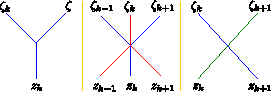
\includegraphics[scale=2]{figures/weaves_types_vertices_ReebCoordinates.pdf}
\caption{The Reeb coordinates above and below each of the weave vertices. \Cref{prop:change_Reebcoordinates_add_vertex_on_top} explains how to relate the bottom Reeb $z$-coordinates and the top Reeb $\zeta$-coordinates.}
    \label{fig:weaves_types_vertices_ReebCoordinates}
\end{figure}

\begin{proposition}\label{prop:change_Reebcoordinates_add_vertex_on_top} In the notation above, the following holds:
\begin{enumerate}[label=$(\roman*)$]
    \item If $p$ is a hexavalent vertex inserted on top of the crossings $\s_{i_{k-1}}\s_{i_{k}}\s_{i_{k+1}}$ of $\beta$, then
    $$z_{k-1}=\zeta_{k+1},\quad z_{k}=\zeta_{k-1}\zeta_{k+1}-\zeta_{k},\quad z_{k+1}=\zeta_{k-1},\quad z_{j}=\zeta_{j}\quad \mbox{if }j\not\in\{k-1,k,k+1\}.$$
    Equivalently, the inverse transformation is
    $$\zeta_{k-1}=z_{k+1},\quad \zeta_{k}=z_{k-1}z_{k+1}-z_{k},\quad \zeta_{k+1}=z_{k-1},\quad \zeta_{j}=z_{j}\quad \mbox{if }j\not\in\{k-1,k,k+1\}.$$

    \item If $p$ is a tetravalent vertex inserted on top of the crossings $\s_{i_{k}}\s_{i_{k+1}}$ of $\beta$, then
    $$\zeta_{k}=z_{k+1},\quad \zeta_{k+1}=z_{k},\quad \zeta_{j}=z_{j}\quad \mbox{if }j\not\in\{k,k+1\}.$$

    \item If $p$ is a trivalent vertex inserted on top of the crossings $\s_{i_{k}}$ of $\beta$, then

$$
\boxed{
\begin{aligned}
\iota^*\left(\zeta_j|_{\{\zeta\neq0\}}\right) & =  z_j \qquad\qquad\quad\mbox{ if } j < k, \\
\iota^*\left(\zeta_k|_{\{\zeta\neq0\}}\right) &=  z_k + t^{-1}, \\
\iota^*(\zeta)&=t,\\
\iota^*\left(\zeta_j|_{\{\zeta\neq0\}}\right) & =  \eta_j(z_1,\ldots,z_{j};t) \mbox{ if } k < j,
\end{aligned}
}
$$
\noindent where $\iota:X(\beta)\times\bG_m\lr X(\beta_+)$ is the embedding induced by the trivalent vertex $p$, with $t\in\bG_m$, the equalities hold in the preimage of the locus $\mbox{im}(\iota)\cong\{\zeta\neq0\}\sse X(\beta_+)$, and we have recursively defined
$$\eta_j(z_1,\ldots,z_{j};t) := \frac{(C_{j-1})_{i_j+1,i_j+1}\cdot z_j - (C_{j-1})_{i_j,i_j+1}}{(C_{j-1})_{i_j,i_j}}, \qquad C_j := B_{i_j}(z_j)^{-1}C_{j-1}B_{i_j}(\eta_j).$$
for $j\in(k,\ell]$ with initial value
$$C_k(t):= \varphi_{i_k} \begin{pmatrix} t & -1 \\ 0 & t^{-1} \end{pmatrix} = \chi_{i_k}(t)x_{i_k}(-t^{-1}) \in \borel.$$
\sbs
\end{enumerate}
\end{proposition}

\noindent \Cref{prop:change_Reebcoordinates_add_vertex_on_top}.$(i)$ and $(ii)$ follow from the $\SL_3$ matrix identities
\begin{equation}
\label{eq: braid moves}
B_i(z_{k-1})B_j(z_k)B_i(z_{k+1}) = B_j(z_{k+1})B_i(z_{k-1}z_{k+1} - z_k)B_j(z_{k-1}),\mbox{ }B_i(z_{k})B_k(z_{k+1}) = B_k(z_{k+1})B_i(z_k).
\end{equation}
in combination with \eqref{eq:braid_var_eq}.
\noindent \Cref{prop:change_Reebcoordinates_add_vertex_on_top}.$(iii)$ is not as local, as \textcolor{blue}{the new trivalent vertex affects all the Reeb coordinates to the right of where it is inserted}, cf.~\cite[Section 5.1]{CGGLSS25}.\footnote{Geometrically, this is due to the nature of the Ng resolution, see \cite[Section 2.1]{Ng03_computable}.} The core $\SL_2$ identity in that case is
\begin{equation}
\label{eq: trivalent}
B_{i_k}(\zeta_k)B_{i_k}(\zeta) = B_{i_k}(\zeta_k - \zeta^{-1})U,\ \quad  U := \varphi_{i_k}\left(\begin{matrix} \zeta & -1 \\ 0 & \zeta^{-1} \end{matrix} \right).
\end{equation}
 

\noindent The equation \eqref{eq: trivalent} is defined only when $\zeta \neq 0$ and can be inserted in the middle of a product of several braid matrices. Thus, from the viewpoint of matrix computations, the reason the Reeb coordinates to the right of $\zeta$ are affected is because we must move the element $U \in \borel$ to the right of all the braid matrices $B_{i_j}(z)$ appearing to the right of $B_{i_k}(\zeta)$ in \eqref{eq:braid_var_eq}. This implies that at every trivalent vertex we must modify all the variables appearing to the right of this vertex.\\

\begin{remark}
In the notation of \cite{CGGJ24,CGGLSS25}, the second equation in \Cref{prop:change_Reebcoordinates_add_vertex_on_top}.$(iii)$ would be written as $z_k=\zeta_k-\zeta^{-1}$.\sbs
\end{remark}

\noindent A conceptually important result, which can be proven by combining \Cref{prop:Avariables_up_new_trivalent} and \Cref{prop:change_Reebcoordinates_add_vertex_on_top}.$(iii)$ is the following identity:

\begin{theorem}[in progress]\label{thm:leading_monomial_cluster_A_variables}
Let $\w:\beta\to\delta(\beta)$ be a Demazure weave, $v\in\w$ a trivalent vertex and $\top(\rho_v)\in\N^\ell$ the top weights of the dual Lusztig cycle $\rho_v$. Then the leading monomial of $A^\w_v(z_1,\ldots,z_\ell)$ in the lexicographic order $z_1\prec z_2\prec \ldots\prec z_\ell$ is ${\bf z}^{\top(\rho_v)}$.\sbs
\end{theorem}

\noindent In \Cref{thm:leading_monomial_cluster_A_variables} we used the notation ${\bf z}^{\vec{a}}:=z_1^{a_1}\ldots z_\ell^{a_\ell}$ if $\vec{a}:=(a_1,\ldots,a_\ell)\in\N^\ell$. In the statement, we also implicitly lifted a regular function $A^\w_v(z_1,\ldots,z_\ell)\in\Z[X(\beta)]$ to an actual polynomial, as a regular function in an ambient affine space. There are choices of such lifts, but the scanning of Demazure weaves gives a natural one, which is the one we work with, cf.~\cite[Section 7.2]{CGGLSS25}.

%%%%%%%%%%%%%%%%%%%%%%%%%%%%%%%%%%%%%%%%%%%%%
%%%%%%%%%%%%%%%%%%%%%%%%%%%%%%%%%%%%%%%%%%%%%
\subsection{Hook content formula for cluster $A$-variables}\label{ssec:hook_content_formula} Let $\w:\beta\to\delta(\beta)$ be a Demazure weave and $v\in\w_3$ a trivalent vertex. By \Cref{thm:polynomiality}, $A_v(z)$ is a polynomial in the Reeb $z$-coordinates and, by \Cref{thm:leading_monomial_cluster_A_variables}, the exponents of its leading term are captured by $\top(\rho_v)$. It could be desirable to have a way to compute the entirety of the polynomial $A_v(z)$, with all its monomials and their coefficients, in terms of the combinatorics of the weave $\w$.\\

In order to establish such formula, one must work with raked weaves as in \cite[Section 5.1]{CGGLSS25} and introduce some variations on the dual Lusztig cycle $\rho_v$, which are indexed by bonsai forests (\begin{CJK*}{UTF8}{min}
寄せ植え
\end{CJK*}, yose--ue). A bonsai forest $\mathsf{y}$ involves a choice of certain rooted trees, the bonsais, along each rake of the weave. Such a choice of bonsais along each rake dictates an upwards propagation from $v$, leading to a Lusztig-like weave cycle $\rho_{\mathsf{y}}$ on $\w$. Each bonsai forest $\mathsf{y}$ has a hook content $h(\mathsf{y})$ obtained by multiplying the hooks of certain vertices in its bonsai trees. Let us denote by $\mathsf{F}_v(\w)$ the set of bonsai forests associated to a trivalent vertex $v\in\w_3$. The cluster $A$-variables of a Demazure weave can be expressed combinatorially in terms of the Reeb coordinates as follows:

\begin{theorem}[Hook content formula]\label{thm:hook_content_cluster_A_variables}
Let $\w:\beta\to\delta(\beta)$ be a Demazure weave, $v\in\w$ a trivalent vertex and $A^\w_v(z_1,\ldots,z_\ell)$ the cluster $A$-variable of $v$ in terms of Reeb coordinates. Then
\begin{equation}\label{eq:hook_formula}
\boxed{A^\w_v(z_1,\ldots,z_\ell)=\sum_{\mathsf{y}\in\mathsf{F}_v(\w)} \frac{z^{\on{top}(\rho_{\mathsf{y}})}}{h(\mathsf{y})} }
\end{equation}
where the sum is taken over the collection of bonsai forests starting at $v$.\sbs
\end{theorem}

\noindent There is currently no proof of \Cref{thm:hook_content_cluster_A_variables} printed in the literature, though it can be deduced from the relation between spectral networks and Floer theory as developed in \cite{casals2025spectralnetworksbettilagrangians}. Hopefully a more direct proof of \eqref{eq:hook_formula}, without using \cite{casals2025spectralnetworksbettilagrangians}, will appear within the next year. In terms of \eqref{eq:hook_formula}, it is not clear that the polynomial $A^\w_v(z_1,\ldots,z_\ell)$ has integral coefficients, as the sum occurs with rational coefficients. That said, it follows from the construction of \cite[Section 7.2]{CGGLSS25}, which is well-defined over $\Z$, that $A^\w_v(z_1,\ldots,z_\ell)$ must have integral coefficients. It would be enlightening to have a combinatorial proof of this fact.

%%%%%%%%%%%%%%%%%%%%%%%%%%%%%%%%%%%%%%%%%%%%%
%%%%%%%%%%%%%%%%%%%%%%%%%%%%%%%%%%%%%%%%%%%%%
\subsection{The torus action in the Reeb coordinates}\label{sssec:torus_action_coordinates} For $\G=\SL_n$, the torus action \eqref{eq:torus_action} from \Cref{sssec:braid_variety_further_symmetries} can be written in the Reeb $z$-coordinates explicitly, as established in \cite[Section 2.2]{CGGJ24}. The statement reads as follows:

\begin{lemma}[$\T$-action in Reeb coordinates]\label{lem:torusaction_coordinates} The $\T$-action on $X(\beta)$ from \cref{eq:torus_action}
$$\T\times X(\beta)\lr X(\beta),\quad (\tau;\borel_1,\borel_2,\dots, \borel_{\ell+1})\mapsto (\tau\borel_1,\tau\borel_2,\dots, \tau\borel_{\ell+1})$$
is expressed in the $z$-coordinates for $X(\beta)$ as
$$
(t;z_1,\ldots,z_{\ell}):=(\color{blue}t_{w_1(i_{1})}\color{black}z_1\color{blue}t^{-1}_{w_1(i_{1}+1)}\color{black},\color{blue}t_{w_2(i_{2})}\color{black}z_2\color{blue}t^{-1}_{w_2(i_{2}+1)}\color{black},\ldots,\color{blue}t_{w_{\ell}(i_{\ell})}\color{black}z_{\ell}\color{blue}t^{-1}_{w_{\ell}(i_{\ell}+1)}\color{black}),
$$
%where $c_k(t)$ are given by the formula
%$$c_k=t_{w_k(i_{k}+1)}t^{-1}_{w_k(i_{k})},\quad k\in[1,\ell]$$
\noindent where $w_j:= s_{i_1}\cdots s_{i_{j-1}}\in S_n$ denote the permutations associated to the partial words for $\beta$, $j\in[1,\ell+1]$, and $t\in\T$ and $(z_1,\ldots,z_{\ell})\in \mathbb{A}_\kk^{\ell}$.
%and $w=w_{r+1}$ is the permutation corresponding to $\beta$.
\end{lemma}
\begin{comment}
\begin{proof}
Let us abbreviate $c_k=t_{w_k(i_{k}+1)}t^{-1}_{w_k(i_{k})}$ and consider the diagonal matrix $D(t)$ representing the point $t=(t_1,\ldots,t_n)\in\T$, so its $(i,i)$-entry is $t_i$, $i\in[1,n]$. Then the statement follows from the identity
\begin{equation*}
%\label{eq:slide diagonal 2}
D(t)B_{i_1}(z_1)\cdots B_{i_r}(z_r)=B_{i_1}(c_1z_1)\cdots B_{i_r}(c_rz_r)D(\pi_\beta(t)),
\end{equation*}
where $\pi_\beta=w_{\ell+1}$ is the permutation associated to $\beta$. This identity is implied by the following equality in $\SL_2$:
$$\displaystyle\left(\begin{matrix} t_1 & 0\\ 0 & t_2\\ \end{matrix}\right)\left(\begin{matrix} z & -1\\ 1 & 0\end{matrix}\right)=\left(\begin{matrix}t_1zt_2^{-1} & -1\\
1 & 0\\ \end{matrix}\right)\left(\begin{matrix} t_2 & 0\\ 0 & t_1\\ \end{matrix}\right).$$
\end{proof}
\end{comment}
\noindent Visually, the indices $i_k,j_k\in[1,n]$ of $t_{i_k}z_kt_{j_k}^{-1}$ can be read from the braid diagram as follows, cf.~\cite[Section 2.2]{CGGJ24}. Consider the $k$th crossing in the braid diagram, which has the variable $z_k$ associated to it, and follow the top left strand at that crossing to the left until reaching the beginning of the braid diagram for $\beta$, at its leftmost part. This selects a strand at the leftmost part of the braid diagram $\beta$: the index of that strand is then $j_k$, indexing strands counting from the bottom. Similarly, the index $i_k$ is that of the strand at the leftmost part of the braid diagram for $\beta$ which is reached by following the bottom left strand at the $k$th crossing to the left.

%%%%%%%%%%%%%%%%%%%%%%%%%%%%%%%%%%%%%%%%%%%%%
%%%%%%%%%%%%%%%%%%%%%%%%%%%%%%%%%%%%%%%%%%%%%
\subsection{The cluster 2-form in the Reeb coordinates}\label{sssec:symplectic_form_coordinates} Given a cluster seed $\{A_i\}$ with a skew-symmetric exchange matrix $B=(b_{ij})$ we can consider the following cluster 2-form
\begin{equation}\label{eq:cluster_2form}
\omega_{cl}:=\sum_{i,j}b_{ij}\frac{dA_i\wedge dA_j}{A_iA_j}=\sum_{i,j}b_{ij}\cdot d\log(A_i)\wedge d\log(A_j)
\end{equation}
\noindent in the torus $\Spec \kk[A_1^{\pm1},\ldots,A_\ell^{\pm1}]$ underlying the seed. By the mutation formula for cluster $A$-variables, the 2-forms associated to all the different cluster seeds glue together to give a well-defined global 2-form on (the spectrum of) the cluster algebra. Such cluster 2-form is a central ingredient in the study of symplectic and Poisson structures in relation to cluster algebras, see e.g.~\cite{FG2006,FG09,GSV05,GSV}. The goal of this subsection is to present an expression of the cluster 2-form \eqref{eq:cluster_2form} in terms of the Reeb coordinates.\\

For simplicity, we assume that $\delta(\beta) = w_0$ and $\kk=\C$. Let $\theta^L$ and $\theta^{R}$ denote the left and right invariant $\mathfrak{g}$-valued forms on $\G$, respectively, a.k.a.~the Maurer-Cartan forms. For instance, if $\G = \SL_n$ then we can write $\theta^L(f) = f^{-1}df$ and $\theta^{R}(g) = dg\cdot g^{-1}$ explicitly. Let $\kappa: \mathfrak{g} \otimes \mathfrak{g} \to \kk$ be the (normalized) Killing form on the Lie algebra $\mathfrak{g}$ of $\G$. Consider the following $2$-form on $\G \times \G$:
\begin{equation}\label{eq:fg_pairing}
(f|g) := \kappa(\theta^L(f)\wedge\theta^{R}(g))
\end{equation}
\noindent where $f,g\in\G$. Here \eqref{eq:fg_pairing} defines a skew-symmetric bilinear form at $T_{(f,g)}\G\times\G$ which, when varying the point $(f,g)\in\G\times\G$ defines an element of $\Omega^2(\G\times\G)$. Note that $(\cdot|\cdot)$ as defined in \eqref{eq:fg_pairing} satisfies a cocycle condition:
\begin{equation}
\label{eq: cocycle}
(f|g)+(fg|h)=(f|gh)+(g|h).
\end{equation}
Given a collection of $\G$--valued functions $f_1,\ldots,f_{\ell}$, we define
\begin{equation}
    \label{eq: 2 form}
(f_1|\cdots |f_{\ell}):=(f_1|f_2)+(f_1f_2|f_3)+\ldots+(f_1\cdots f_{\ell-1}|f_{\ell}).
\end{equation}
\noindent By \eqref{eq: cocycle} this definition is associative in the entries $f_i$. Let $\beta=\sigma_{i_1}\cdots\sigma_{i_\ell}$, we relate this construction to the braid variety $X(\beta)$ by applying \eqref{eq: 2 form} with $f_j:=B_{i_j}(z_j)$. Specifically, by using the embedding $X(\beta)\sse\mathbb{A}_\kk^\ell$ given by the Reeb coordinates in \Cref{lem:equations_braidvar} we define:
\begin{definition}\label{def:braid_variety_2_form} Let $\beta=\sigma_{i_1}\cdots\sigma_{i_\ell}$ be a positive braid word and $X(\beta)\sse\mathbb{A}_\kk^\ell$ its braid variety embedded via the Reeb coordinates. By definition, the 2-form $\omega_\beta\in\Omega^2X(\beta)$ is the restriction
\begin{equation}\label{eq:braid2form}
\omega_\beta:=(B_{i_1}(z_1)|\cdots |B_{i_{\ell}}(z_{\ell}))|_{X(\beta)},
\end{equation}
where $(B_{i_1}(z_1)|\cdots |B_{i_{\ell}}(z_{\ell}))\in\Omega^2\mathbb{A}_\kk^\ell$ is a 2-form in the Reeb coordinates.\sbs
\end{definition}
By \Cref{def:braid_variety}, the image of the map $B_{\beta}: \mathbb{A}_\kk^\ell \to \G$ restricted to the braid variety must have its image contained in $\delta(\beta)\borel$. Thus $\omega_\beta$ is a closed 2-form on $X(\beta)$. The following result is \cite[Theorem 9.5]{CGGLSS25}:

\begin{proposition}\label{prop:2forms}
Let $\beta$ be a positive braid word, $X(\beta)$ its braid variety and $\omega_{cl}\in\Omega^2 X(\beta)$ the cluster 2-form defined by any cluster seed coming from a Demazure weave $\w:\beta\to\delta(\beta)$. Then
\begin{equation}\label{eq:equality_2_forms}
\boxed{\omega_\beta=\omega_{cl}}
\end{equation}
\sbs
\end{proposition}

\noindent In particular, since $\omega_\beta$ is defined entirely in terms of the Reeb coordinates, \Cref{prop:2forms} expresses the cluster 2-form $\omega_{cl}$ in terms of the Reeb coordinates.


%%%%%%%%%%%%%%%%%%%%%%%%%%%%%%%%%%%%%%%%%%%%%
%%%%%%%%%%%%%%%%%%%%%%%%%%%%%%%%%%%%%%%%%%%%%
\subsection{The Landau-Ginzburg brick potential in the Reeb coordinates}\label{thm:superpotential_Reeb_coordinates} Building on the brick compactifications $(Y(\beta),D_\beta)$ introduced in \Cref{ssec:brick_compactifications}, we now proceed to computing the potentials $W_\beta$ associated to such compactifications, cf.~\Cref{sssec:applications_compactifications}. Specifically, here the term {\it potential} is understood within the context of Landau-Ginzburg models, see e.g.~\cite[Sections 3\& 11]{GoncharovShen15}, \cite[Sections 3\&4]{GS19} and \cite[Section 0.4]{GHKK18}.\footnote{This use should not be confused with the notion of potentials in the context of {\it quivers with potential}, which is also an important but different aspect of the study of cluster structures in braid varieties, cf.~\cite{CasalsGao24}.} For specificity, let us assume $\delta(\beta)=w_0$.

\begin{remark} As the upcoming discussion involves a form of mirror symmetry, it is paramount to distinguish whether we are working in the affinization of the $\SA$-scheme or that of the $\SX$-scheme, especially because both happen to be isomorphic to the braid variety $X(\beta)$. In addition, the choice of Lie group also needs to be emphasized. Thus, as in \Cref{sssec:applications_compactifications}, we adopt the notation of $\SA_\G(\beta)$ and $\SX_\G(\beta)$ as presented in \Cref{ssec:A_and_X_schemes_weave}.\sbs
\end{remark}

Let us consider the braid variety $\SX_{\G^\vee}(\beta)$ and use the compactification $Y_{\G^\vee}(\beta)=Y(\beta)$ from \Cref{def:brick}, which yields the log Calabi-Yau pair $(Y_{\G^\vee}(\beta),D_\beta)$, cf.~\Cref{prop:logCY}. Following a tenet in mirror symmetry, cf.~\cite[Section 7.3]{HoriVafa} and \cite[Conjecture 1.1]{Auroux07_Tduality}, compactifying $\SX_{\G^\vee}(\beta)$ should correspond to adding the data of a potential in $\SA_{\G}(\beta)$, see also \cite[Section 1]{GHK15} or \cite[Section 5]{GHKK18}. In our case, we consider the opposite cluster ensemble $(\SA_{\G}(\beta),\SX_{\G^\vee}(\beta))$ as in \cite[Section 1.2]{FockGoncharov09_Dilog2}. This opposite ensemble has the negated $p$-map, so that the $\SX$-variables in the cluster $\SX$-seeds are the inverses, and the exchange matrix also acquires an overall negative sign.\footnote{Note that the cluster $\SA$-mutation rule is invariant under such sign change.} This is done because, in general, each of the boundary divisors in $D_\beta$ gives a discrete valuation $-\ord_D$, in the $\max$-tropical convention, but in this case we want to measure $\ord_D$, and thus it suffices to consider the opposite cluster $\SX$-structure. Thus, given an irreducible divisor component $D$ of the compactifying divisor $D_\beta$, we consider the valuation vector
\begin{equation}\label{eq:tropicallabel}
        q_D:=\bigl(-\ord_D(X_v^{-1}\bigr)_v
             =\bigl(\ord_D(X_v)\bigr)_v,
\end{equation}
where the index for the entries runs over the trivalent vertices of $\w$. Here we understand the valuation $\ord_D:\kk(\SX_{\G^\vee}(\beta))\lr\Z\cup\{\infty\}$ as defining $q_D$, whose entries are seen as tropical points in $\SX_{\G^\vee}(\beta)$, i.e.~as elements of $\SX_{\G^\vee}(\beta)(\Z^T)$. Following \cite[Corollary 11.9]{GHKK18}, we define the potential
\begin{equation}\label{eq:superpotential}
W_{Y(\beta)}:\SA_\G(\beta)\lr\mathbb{A}^1_\kk, \qquad W_{Y(\beta)}:=\sum_{j}\tht_{q_{D_j}},
\end{equation}
where the index $j$ runs over the positions $j\in[1,\ell]$ such that $\delta(\beta\setminus \sigma_{i_j})=\delta(\beta)$, cf.~\Cref{lem:boundary_div}.(1), and the theta functions $\vartheta_{q_D}$ in \eqref{eq:superpotential}, associated to a divisorial valuation $q_D$, are defined as in \cite[Definition 3.3]{GHKK18}. The following result expresses the potential \eqref{eq:superpotential} in terms of the Reeb coordinates:

\begin{theorem}\label{thm:superpotential_Reeb_coordinates} Let $\beta\in\brn$ be a positive braid word, $(\SA_\G(\beta),\SX_{\G^\vee}(\beta))$ its opposite cluster ensemble and $(Y_{\G^\vee}(\beta),D_\beta)$ the brick compactification of $\SX_{\G^\vee}(\beta)$. Then:
\begin{enumerate}
    \item For every non-empty divisor $D_j$ in $D_\beta$,
    \begin{equation}\label{eq:individual}
       \tht_{q_{D_j}}=z_j,
    \end{equation}
where $z_j$ is the $j$th Reeb coordinate of $\SA_\G(\beta)$.\\

\item The potential associated to the compactification $(Y_{\G^\vee}(\beta),D_\beta)$ satisfies
\begin{equation}\label{eq:superpotential_Reeb_coordinates}
 \boxed{\displaystyle
 W_{Y(\beta)}=\sum_{j}z_j}
\end{equation}
where the index runs over $j\in[1,\ell]$ such that $\delta(\beta\setminus \s_{i_j})=\delta(\beta)$.\sbs
\end{enumerate}
\end{theorem}

Note that \eqref{eq:superpotential_Reeb_coordinates} is independent of any choice of the Demazure weave. With regards to \Cref{thm:superpotential_Reeb_coordinates}.(1), there in fact exists a Demazure weave $\w$ whose associated cluster $\SX$-seed is such that the vector $(\ord_{D_j}X_v)_v$ is integral and primitive, with non-negative entries at the mutable vertices, and the Reeb coordinate $z_j$ is the cluster monomial with this exponent vector. About \cref{thm:superpotential_Reeb_coordinates}.(2), note that the coordinate $z_j$ vanishes identically on $X(\beta)$ if $\delta(\beta\setminus\s_{i_j})\neq \delta(\beta)$. Thus \eqref{eq:superpotential_Reeb_coordinates} in \Cref{thm:superpotential_Reeb_coordinates} can be written as
\begin{equation}\label{eq:superpotential_Reeb_coordinates2}
\displaystyle
 W_{Y(\beta)}=\sum_{i=1}^{\ell(\beta)}z_i.
\end{equation}
\Cref{thm:superpotential_Reeb_coordinates} can be proven with the same strategy as \cite[Section 5.5]{CGGLSS25}. Namely, one first computes directly with a weave as in \cite[Figure 16 (left)]{CGGLSS25} in order to deduce \Cref{thm:superpotential_Reeb_coordinates}.(1) for the first Reeb coordinate $z_1$, and then applies cyclic rotations to deduce the statement for the remaining $z_i$ coordinates.

\begin{remark} For reference, a version of \Cref{thm:superpotential_Reeb_coordinates}.(2) was discussed by one of the research groups at the AIM Workshop ``Cluster algebras and braid varieties'' (2023). I recently talked with D.~Weng, one of the active participants in that group, about whether the result would be written anywhere by that group. After that conversation, there seems to be some merit in at least recording a precise statement, for reference, as done in \Cref{thm:superpotential_Reeb_coordinates} above.\sbs
\end{remark}